\subsection{Historia}

Na początku XX wieku, gdy sieci telekomunikacyjne dopiero się rozwijały, wszystkie połączenia zestawiane były ręcznie. W momencie, gdy abonent podnosił słuchawkę telefonu, jego aparat wysyłał sygnał do lokalnej centrali telefonicznej. Na tablicy świetlnej zapalała się lampka informująca telefonistkę o próbie połączenia. Telefonistka odbierała, pytając, z kim abonent chce się połączyć. Następnie wprowadzała odpowiednią wtyczkę do odpowiedniego gniazda na tablicy rozdzielczej, zestawiając fizyczne połączenie między dwoma liniami. Jeśli rozmowa miała się odbyć na większą odległość (np. między miastami) połączenie przekazywane było przez kolejne centrale. Każda centrala po drodze wymagała ręcznej obsługi przez pracujące w nich telefonistki. 

\begin{figure}[!h]
    \centering 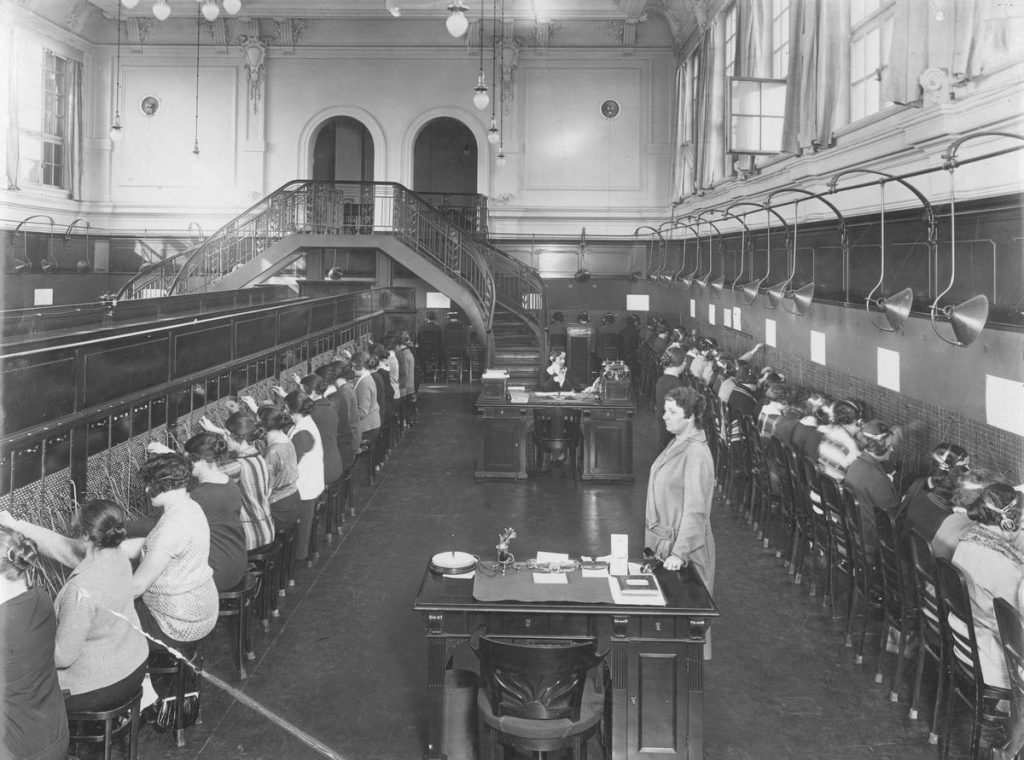
\includegraphics[width=1\linewidth]{telefonistki.jpg}
    \caption{Pracowniczki warszawskiej centrali telefonicznej na zdjęciu z końca lat 20. (domena publiczna).}\label{fig:telefonistki}
\end{figure}

Dziś taki scenariusz wydaje się wręcz absurdalny, a oferty pracy dla telefonistek dawno już zniknęły z tablic ogłoszeń. Praca wykonywana przez telefonistki (czyli komutacja łączy) nadal jest potrzebna do prawidłowego funkcjonowania sieci telekomunikacyjnych, lecz wykonywana jest przez programy komputerowe w sposób w pełni zautomatyzowany. Ręczna komutacja była pierwszym krokiem w kierunku rozwoju globalnych sieci telekomunikacyjnych i choć z dzisiejszej perspektywy wydaje się być bardzo pracochłonna i ograniczająca, bez niej nie powstałyby fundamenty, na których oparto późniejsze systemy automatyczne. Jest to przykład tego, jak technologia stopniowo uwalniała człowieka od bezpośredniej obsługi różnych systemów (dając mu przestrzeń na rózwój w innych obszarach). 

Na zasadzie indukcji możemy przyjąć, iż dziś znajdujemy się w podobnym położeniu - sieci telekomunikacyjne wciąż wymagają bezpośredniego zarządzania przez człowieka. Po prostu granica tego styku - system-człowiek - jest mocno przesunięta. Dziś człowiek spotyka się z systemami dużo bardziej złożonymi, a zarazem dającymi dużo więcej możliwości. Możliwe, że nie istnieje ostateczny punkt styku i systemy telekomunikacyjne zawsze będą wymagały nadzoru ludzkiego. Niezależnie od tej kwestii przesunięcie tej granicy w czasach telefonistek, a dziś wymaga automatyzacji innego rodzaju. 

O telefonistkach możemy powiedzieć, że zarządzały one pracą systemu telekomunikacyjnego \footnote{t.j. siecią PSTN}. Regulowały one jego działanie. W momencie zgłoszenia zastawały one system w pewnym stanie i w ramach realizacji zgłoszenia musiały doprowadzić system do nowego (docelowego) stanu. Cała ich praca tak naprawdę polegała na "wnioskowaniu" (ang. \textit{reason}) jak ma wyglądać stan docelowy, a następnie na wykonaniu \textit{akcji}, która doprowadzała system do tego stanu. 

\begin{figure}[!h]
    \centering 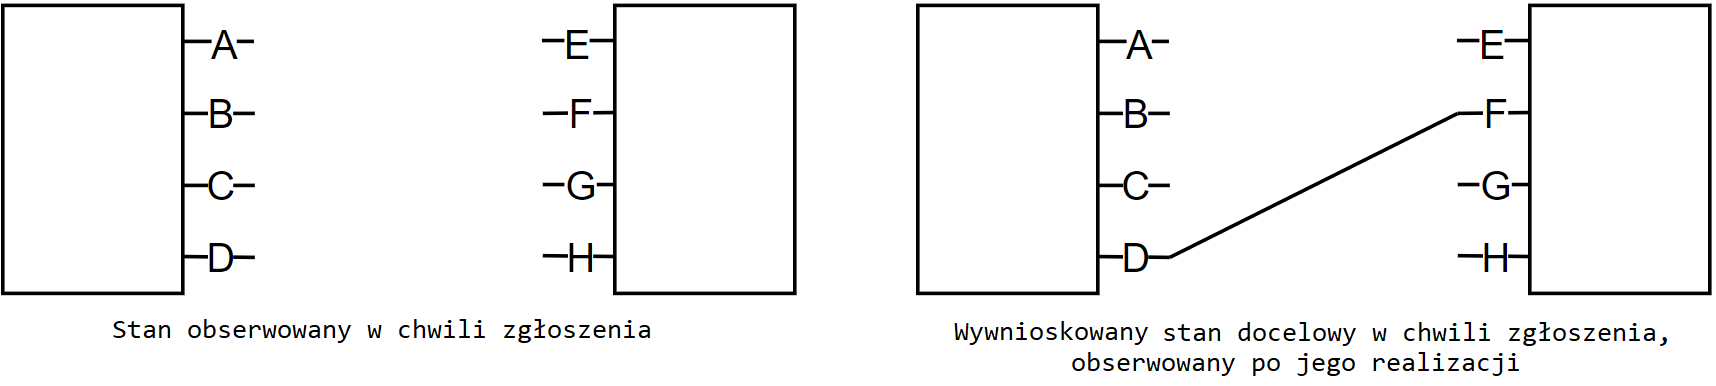
\includegraphics[width=1.0\linewidth]{22-system.png}
    \caption{Dwa stany systemu: sprzed, oraz po realizacji zgłoszenia o treści: "D" chce zadzwonić do "F"}\label{fig:}
\end{figure}

Pomówmy trochę o \textit{wnioskowaniu}. Jak ono przebiega? Po pierwsze telefonistka otrzymuje \textit{dane}. Dane są to fakty lub statystki zebrane razem w celu analizy. Telefonistka zbiera dane w formie faktów jakie miały miejsce. Zadzwonił aparat telefoniczny, telefonistka podniosła słuchawkę i usłyszała w niej, że abonent chce się połączyć ze swoim szwagrem mieszkającym w kamienicy pod numerem 35 na ulicy polnej. Dostępne dane, telefonistka przekuła na \textit{informację}. Informacja to dane pozbawione formy przekazu. Równie dobrze, rozmowa z abonentem mogła przebiec zupełnie inaczej lub telefonistka mogła by otrzymać listowną prośbę o realizację połączenia. Zupełnie inne dane dostarczyły by tej samej informacji, czyli to, że abonent spod konkretnego łącza, chce się dodzwonić do abonenta spod innego, konkretnego łącza. Gdy telefonistka otrzyma informacje na temat zgłoszenia, łączy ją z dotychczasowo posiadanymi informacjami, jak rozmieszczenie łączy na tablicy komutacyjnej. Następnie używa swojej \textit{wiedzy}, czyli zestawu wzorców, które pozwalają jej wytłumaczyć oraz przewidzieć co się wydarzyło, dzieje w tej chwili lub może wydarzyć w przyszłości. Wiedza opiera się na informacji oraz umiejętnościach pozyskanych dzięki doświadczeniu lub edukacji.  Obserwuje ona aktualny stan systemu i \textit{rozumując}, na podstawie wiedzy wyobraża sobie stan docelowy (pożądany) oraz definiuje \textit{akcje}, jakie należy przeprowadzić na systemie, aby osiągnął on ten stan. 


W przypadku komutacji proces wnioskowania jest względnie prosty, dający się do zapisania w języku programowania. Dlatego też wraz z rozwojem technologicznym dokonano przejścia na automatyczne centrale telefoniczne. Jednakże opis wyżej nadal pozostaje ważny. Do centrali trafiają dane w postaci sygnału na jednym z łącz. Sygnał przedstawia numer MSISDN abonenta końcowego. Centrala przekuwa te dane na informacje, a następnie program w jej pamięci dokonuje wnioskowania. Dzięki programowalnym przełącznicom komutacyjnym również wykonanie \textit{akcji} (czyli połączenie ze sobą dwóch łączy) jest możliwe bez udziału człowieka. W dzisiejszych czasach proces wnioskowania wykonywany przez ludzi nadzorujących system telekomunikacyjne już nie jest tak prosty. Dzięki wirtualizacji i programowalności funkcji sieciowych każdy rodzaj rozumowania jaki można skondensować do programu komputerowego został już poddany temu procesowi. Teraz akcje wykonywane przez człowieka rzeczywiście wymagają jego inteligencji \footnote{lub sprawczości w świecie fizycznym, której komputerom brakuje}. Dlatego więc następnym krokiem w rozwoju telekomunikacji jest stworzenie inteligentnych sieci. 